% Activate the following line by filling in the right side. If for example the name of the root file is Main.tex, write
% "...root = Main.tex" if the chapter file is in the same directory, and "...root = ../Main.tex" if the chapter is in a subdirectory.
 
%!TEX root =  TMTinderSee.tex

\chapter[Hauptteil]{Hauptteil}

\section{Versuchsplanung}

\subsection{Kartierung}
    Alle Kartierungsvorgänge wurden mit der Free Open Source Software\\
\emph{QGIS}\cite{qgis}durchgeführt.
\begin{figure}[ht]
    \centering
    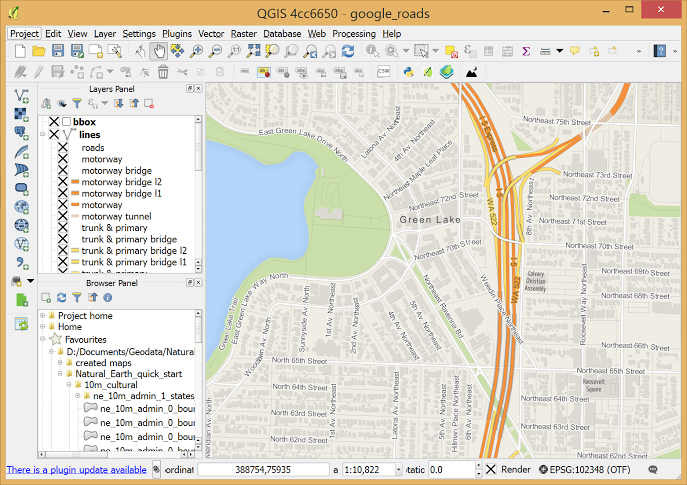
\includegraphics[width=.4\linewidth]{Bilder/QGIS/about-screenshot.png}
    \caption[fig:qgisabout]{QGIS-Benutzeroberfläche}
\end{figure}
\\Mithilfe dieser Software lassen sich basierend auf bereits existierenden Karten, 
wie beispielsweise \emph{OpenStreetMap}\cite{ostrm} oder \emph{OpenSeaMap}\cite{oseam},
eigene Routen und Points of \\Interest(POIs) ohne großen Aufwand eintragen. Genauso 
leicht erfolgt der Import sowie vom Multibeam,  als auch von den Navigationsgeräten 
der ALDEBARAN gespeicherten Positions- und Geschwindigkeitsdaten.\\


Basierend auf dem QGIS-Projekt von \jens, welches die \emph{OpenStreetMap}, sowie den Munitionslagerstättendaten von den Webseiten
\emph{AmuCad}\cite{amucad} und \emph{Munition im Meer}\cite{muninmeer}
als Basis benutzt, konnten wir unsere Route planen (vgl. Abbildungen \ref{fig:route} und \ref{fig:multibeam_route}).

\begin{figure}[]
    \centering
    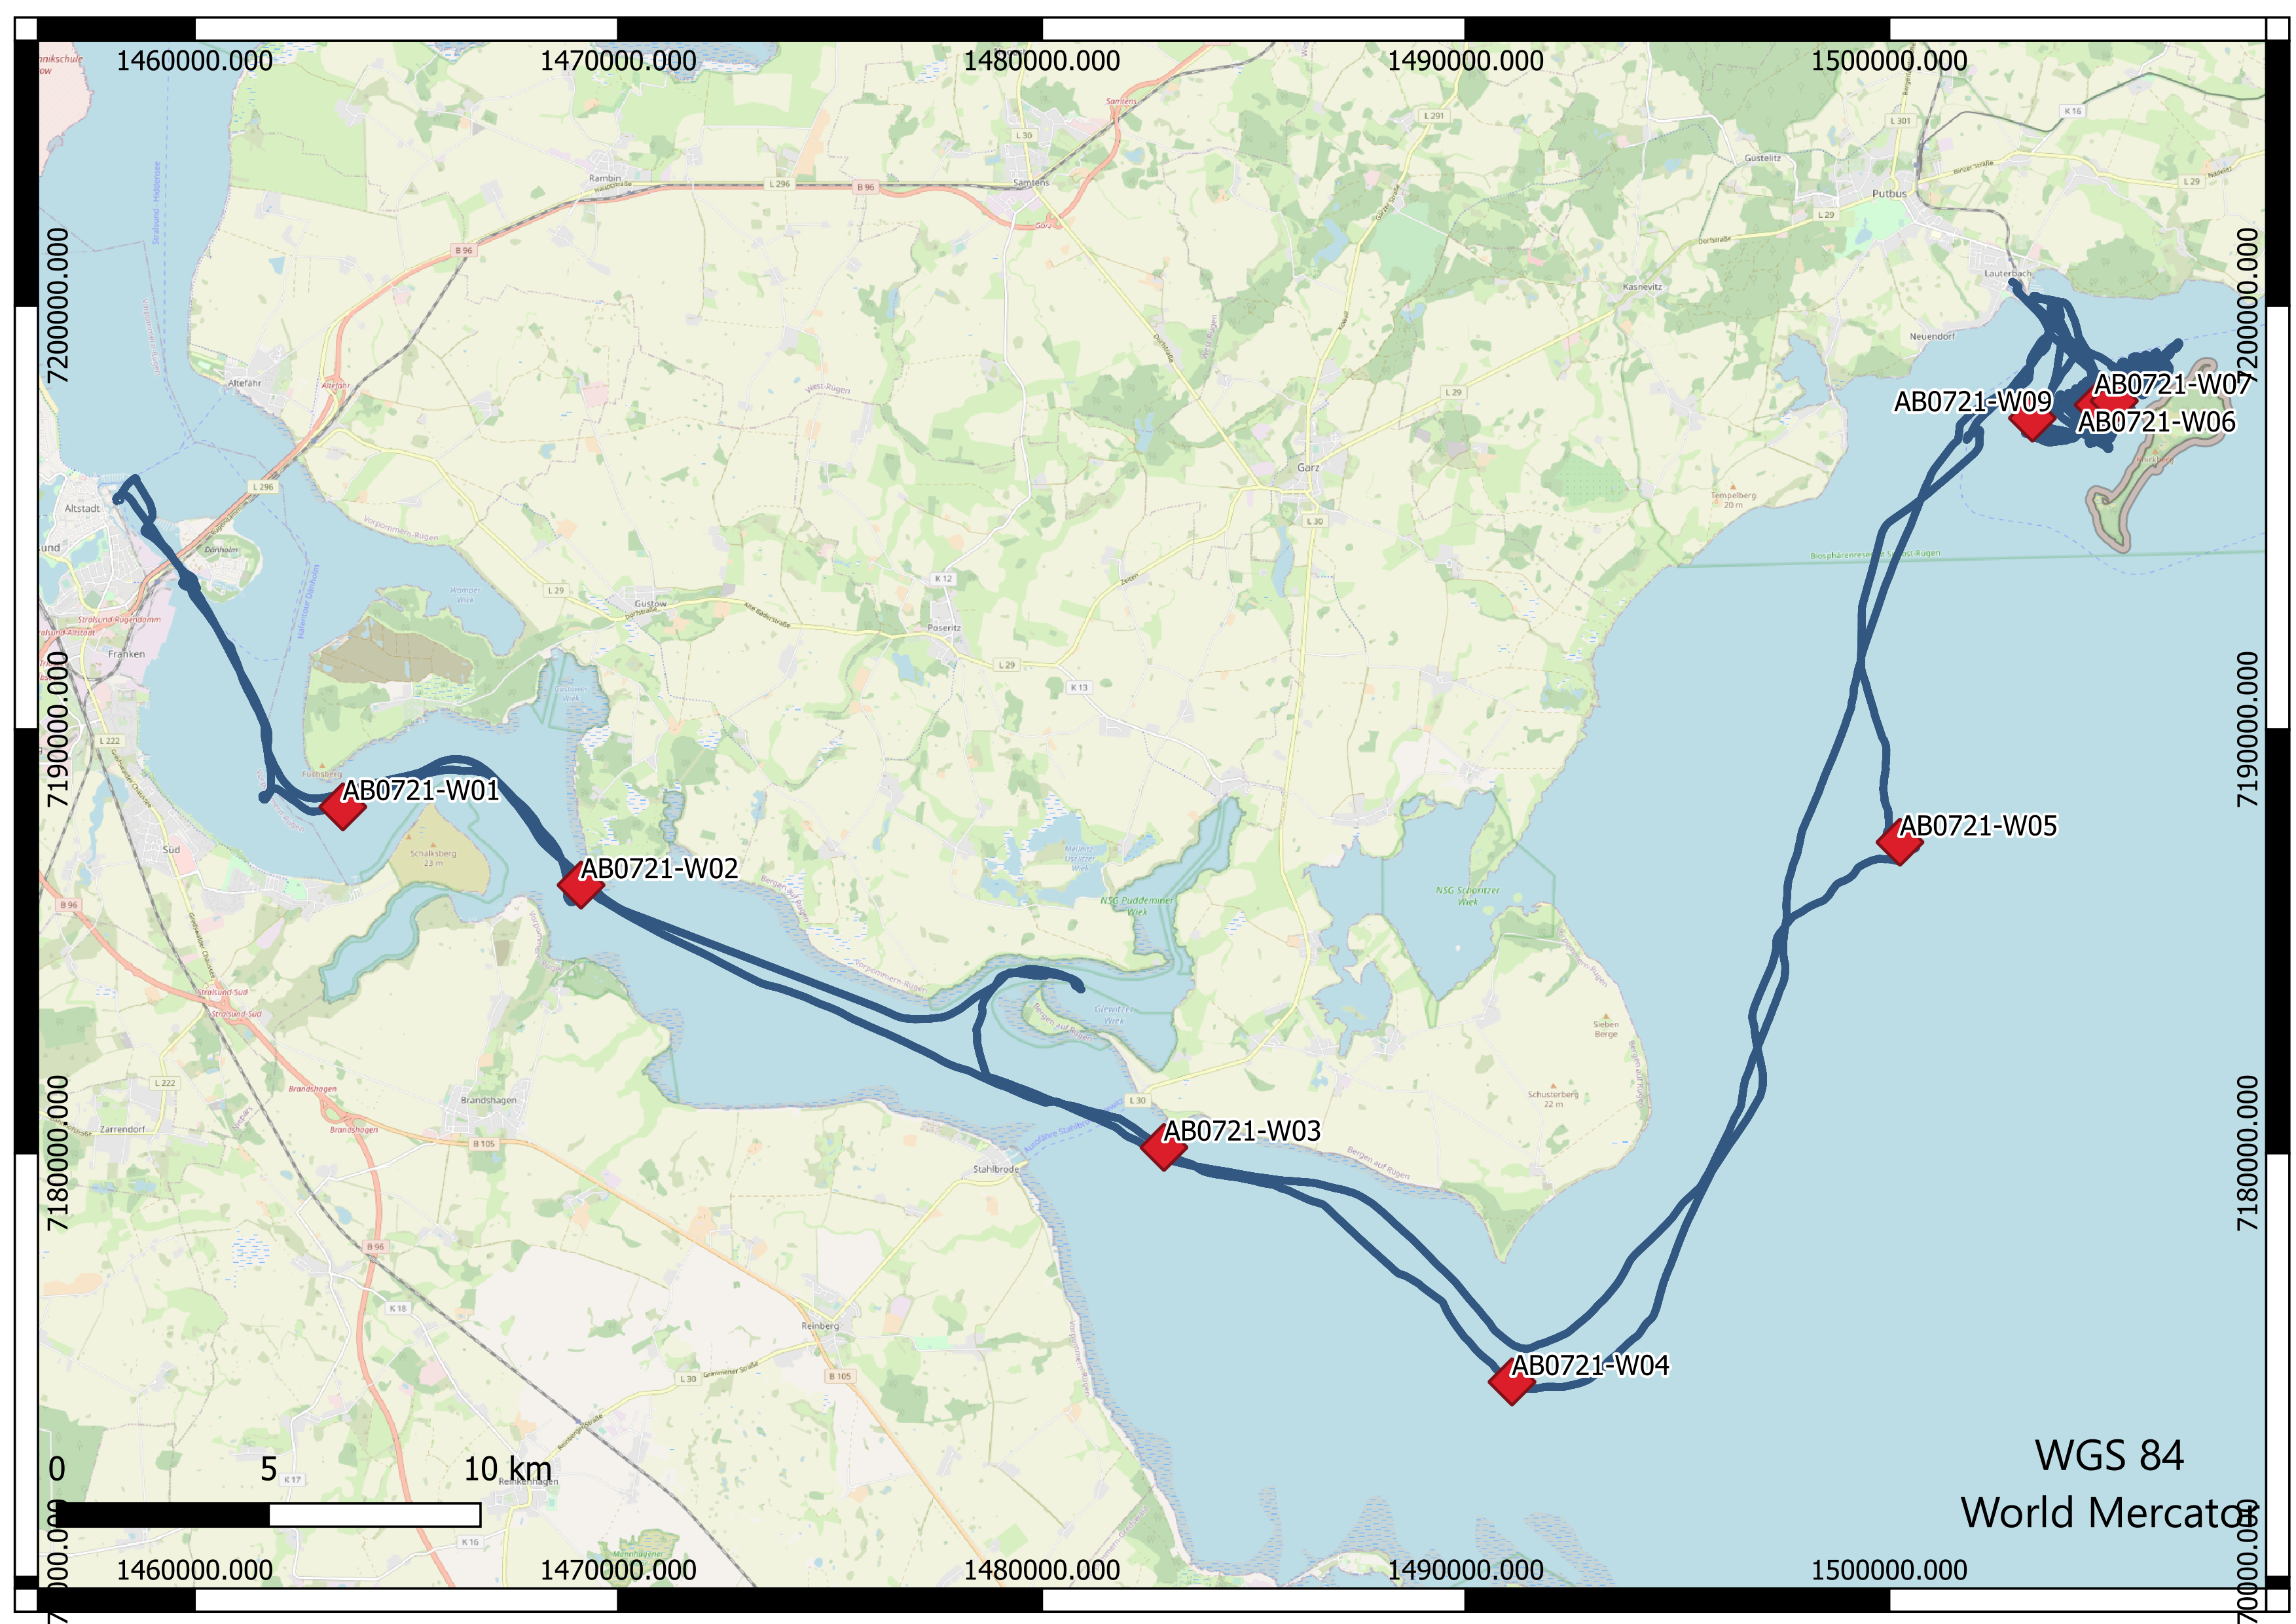
\includegraphics[width=0.8\linewidth]{Bilder/QGIS/Gesamte_route.png}
    \caption{Gesamte Route}
    \label{fig:route}
\end{figure}
\begin{figure}[]
    \centering
    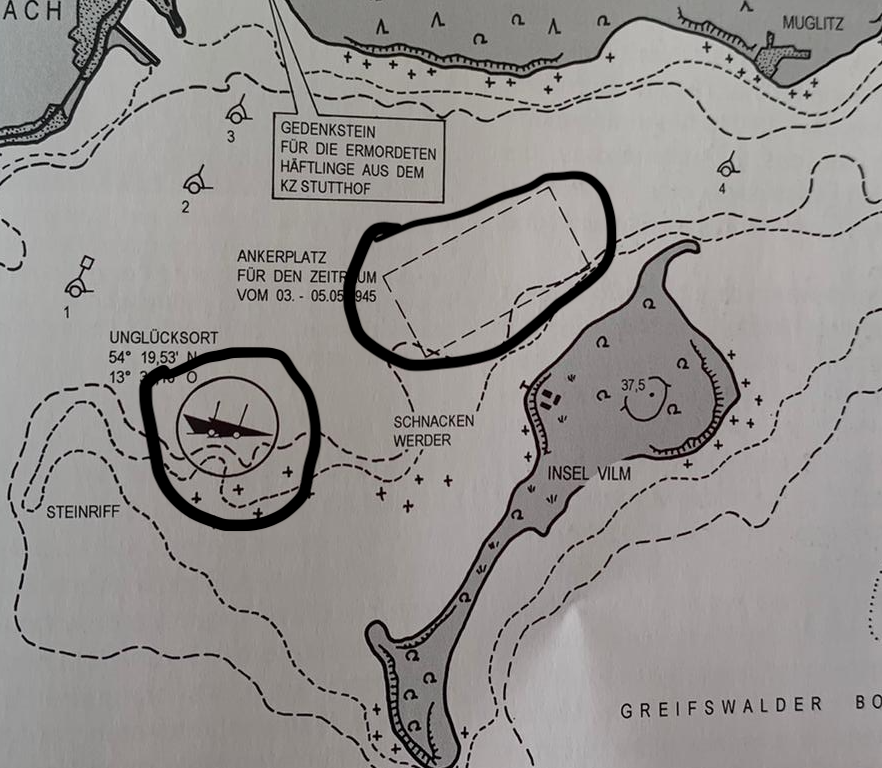
\includegraphics[width=0.8\linewidth]{Bilder/ungl.png}
    \caption{Dokumentierte Anker und Unglückstelle der Sprengstoffschuten.\cite{schiffsschicksale}}
    \label{fig:unglueck}
\end{figure}
\begin{figure}
    \centering
    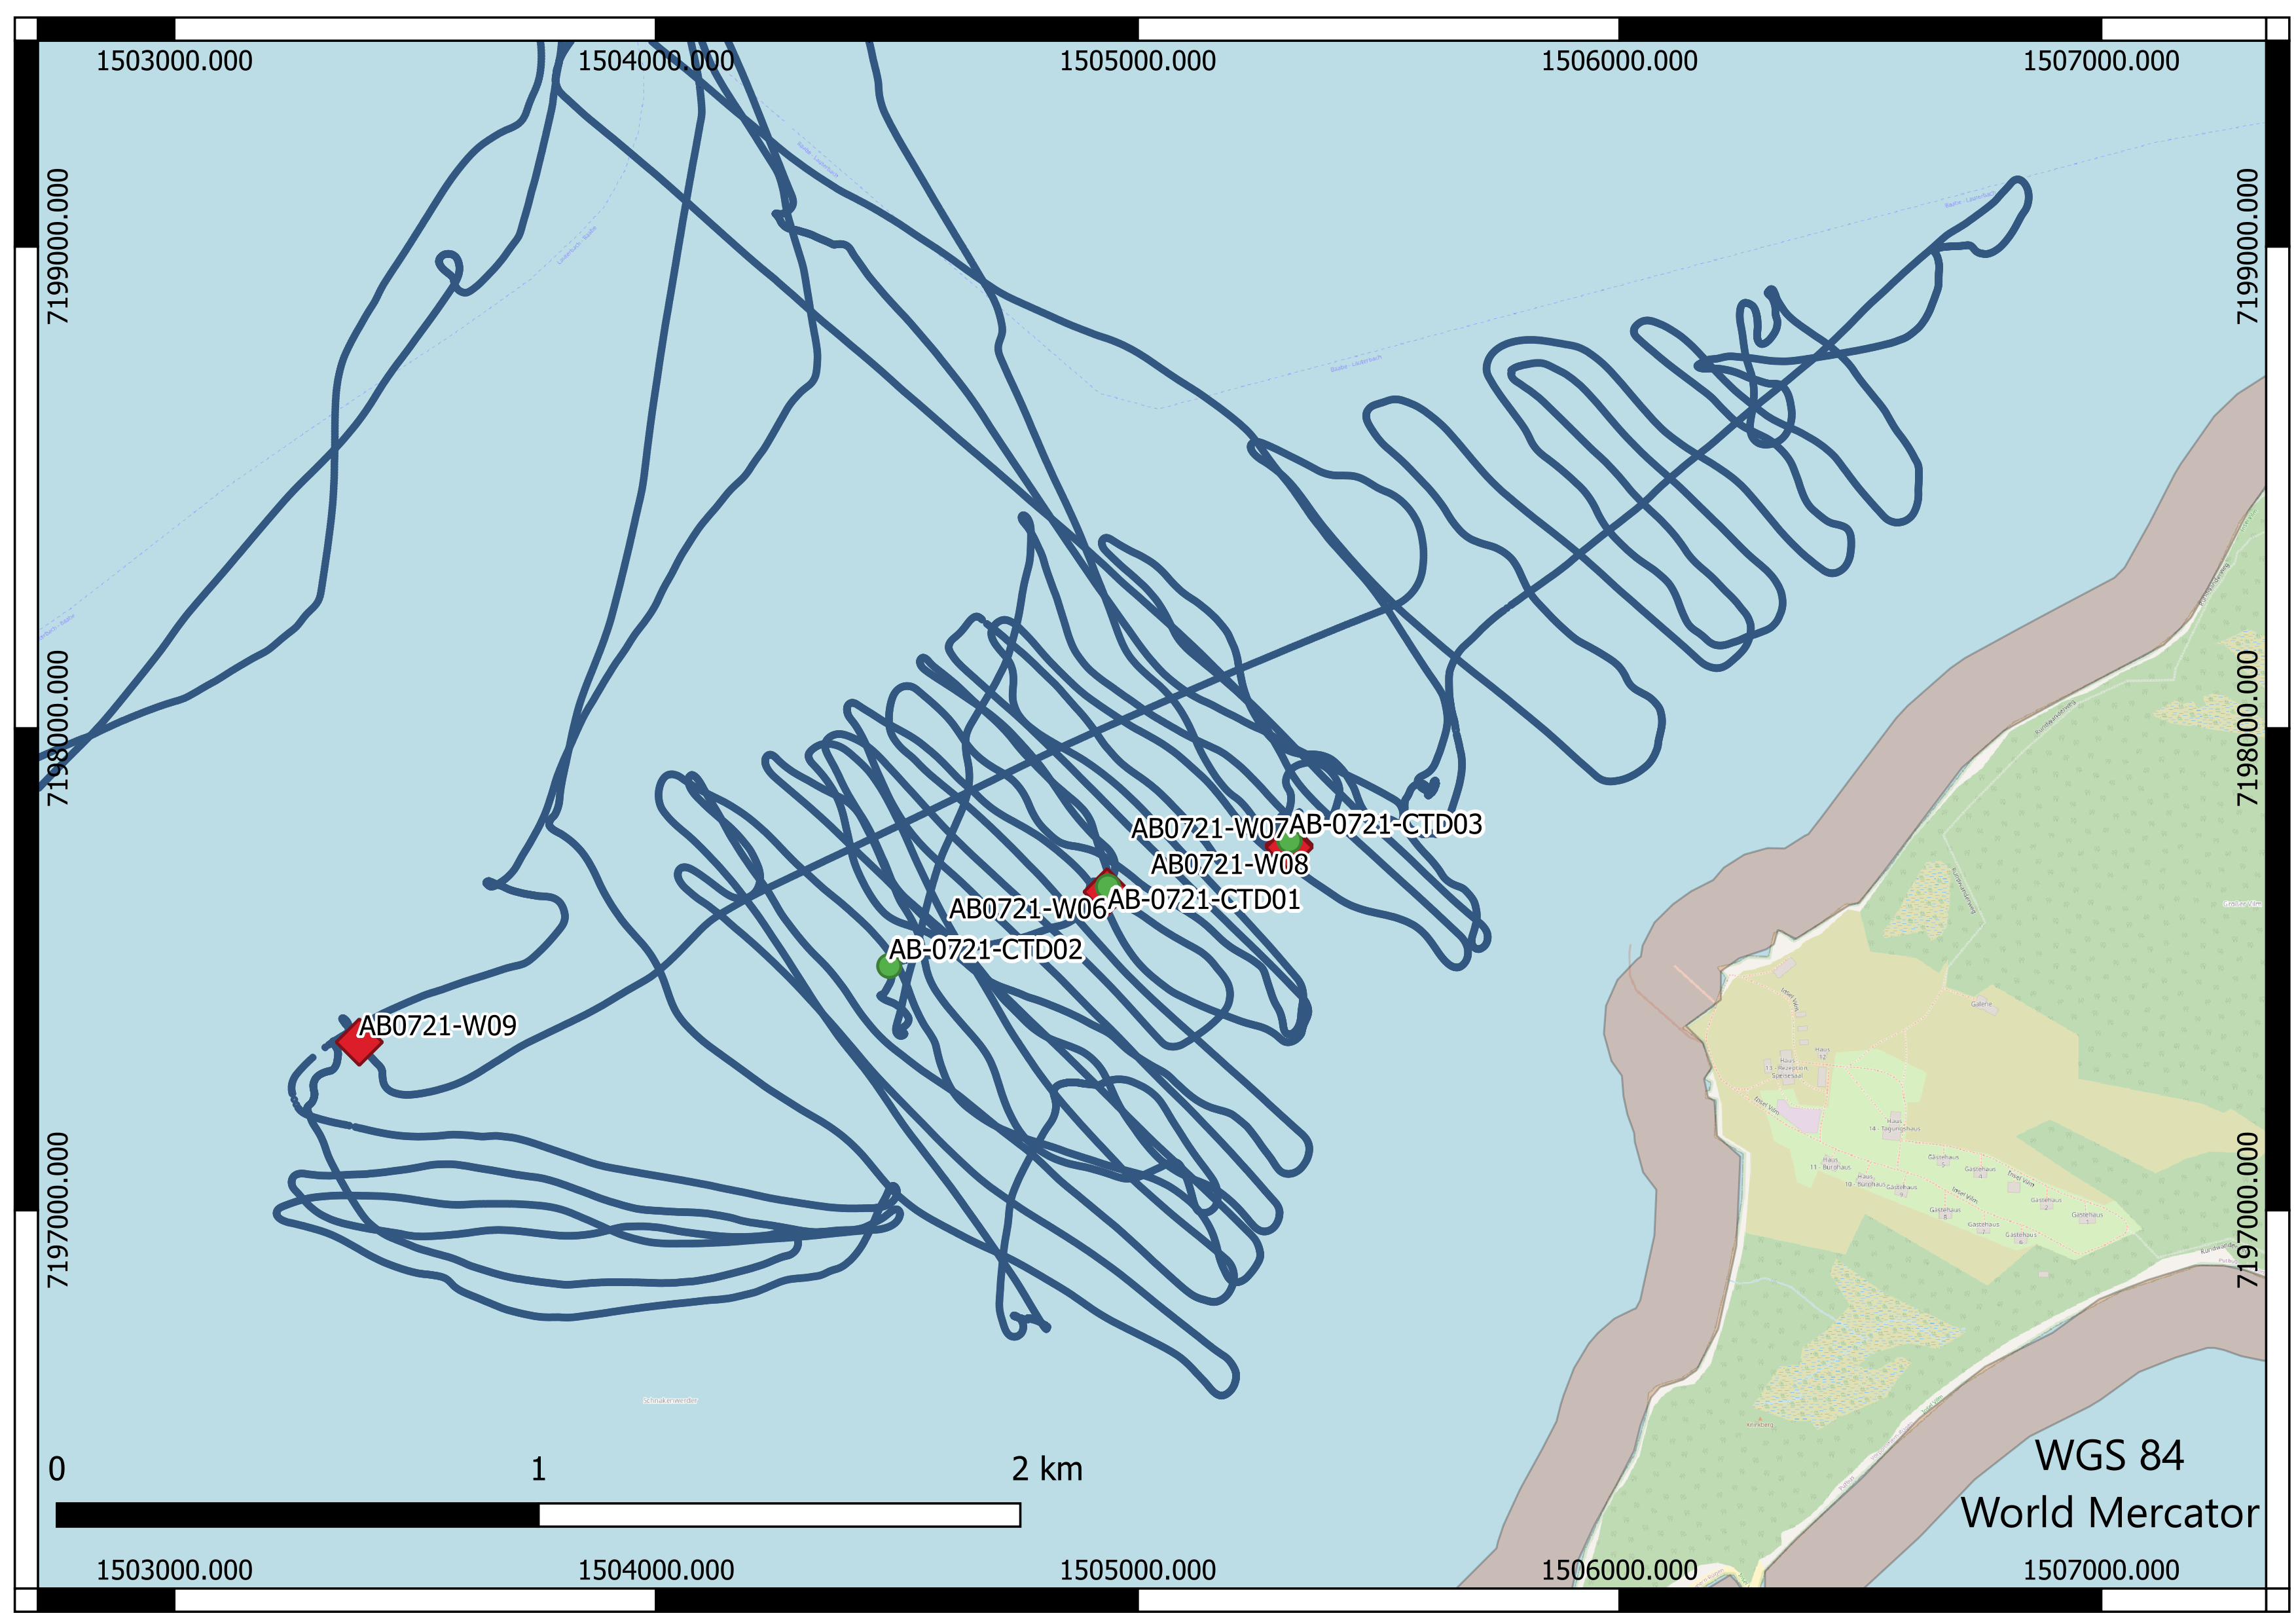
\includegraphics[width=0.8\linewidth]{Bilder/QGIS/multibeam.png}
    \caption{Multibeamfahrten. Wasserproben- und CTD-Stellen sind\\jeweils rot und grün markiert.}
    \label{fig:multibeam_route}
\end{figure}

    
\subsection{Wasserproben}
\subsection{Sedimentproben}
\subsection{Multiparametermessungen}
\subsection{ROV-Kartierungen}

\section{Ergebnisse}
\section{Diskussion der Ergebnisse}

